% !TEX ../report.tex

Ce rapport présente l'application Android \easypass{} conçue dans le cadre du cours MSE \guillemets{MobOp}. 

\section{Concept}

\easypass{} est une application de gestion de mots de passe. 

Tout comme ses concurrents (\emph{LastPass}, etc.), il permet de stocker de manière sécurisée ses mots de passe et de les consulter depuis n'importe où au moyen d'un unique \emph{Master Password}. L'originalité et l'avantage d'\easypass{{} repose dans la manière dont il stocke les informations. 

\includeFigure{1}{intro}{Slides présentés au lancement de l'application.}

\emph{LastPass} par exemple possède ses propres serveurs, tandis que d'autres ont opté pour un stockage local, sur l'ordinateur de l'utilisateur. Dans le premier cas, il est nécessaire d'avoir une confiance totale dans les serveurs du service. Dans le second cas, un accident et nous perdons nos mots de passe (à moins de maitriser l'art de la sauvegarde, ce qui n'est pas si courant).

\easypass{} a opté pour une solution hybride: tous les mots de passe sont sauvegardés dans un simple fichier synchronisé sur \emph{Dropbox}. Ce dernier se charge d'en assurer les sauvegardes et tant qu'un ordinateur est lié au service, une copie locale existe également!

% Stocker des mots de passe sur \emph{Dropbox}... Est-ce sécurisé ? \\
Pour assurer la sécurité des mots de passe, le contenu du fichier est chiffré en utilisant l'algorithme de chiffrement AES~CBC~256. Cet algorithme est pour l'instant considéré comme \guillemets{strong}, mais a également un autre avantage: il est supporté par de nombreux logiciels, notamment \code{openssl}. Ainsi, même si \easypass{} est indisponible ou présente un bug, l'utilisateur peut à tout moment récupérer ses informations en tapant une simple ligne dans son terminal ou un autre outil de la suite \easypass.

% 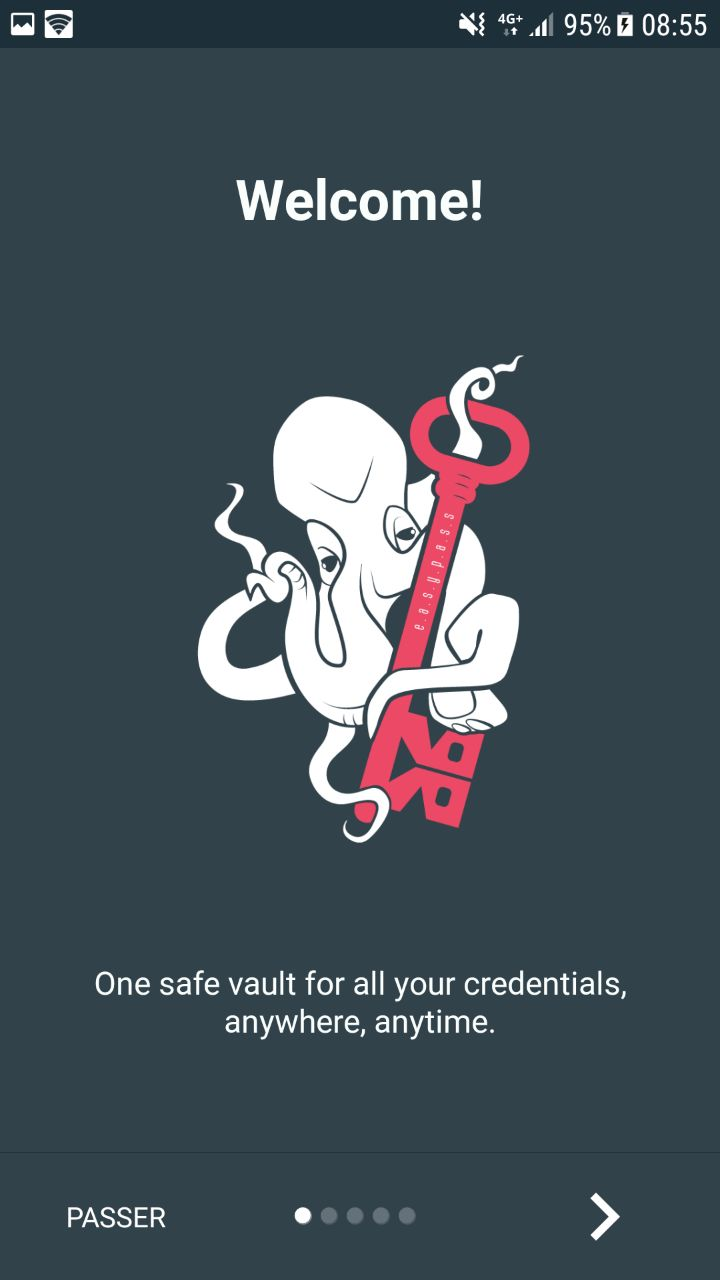
\includegraphics[width=.2\textwidth]{intro-1.jpg}
% 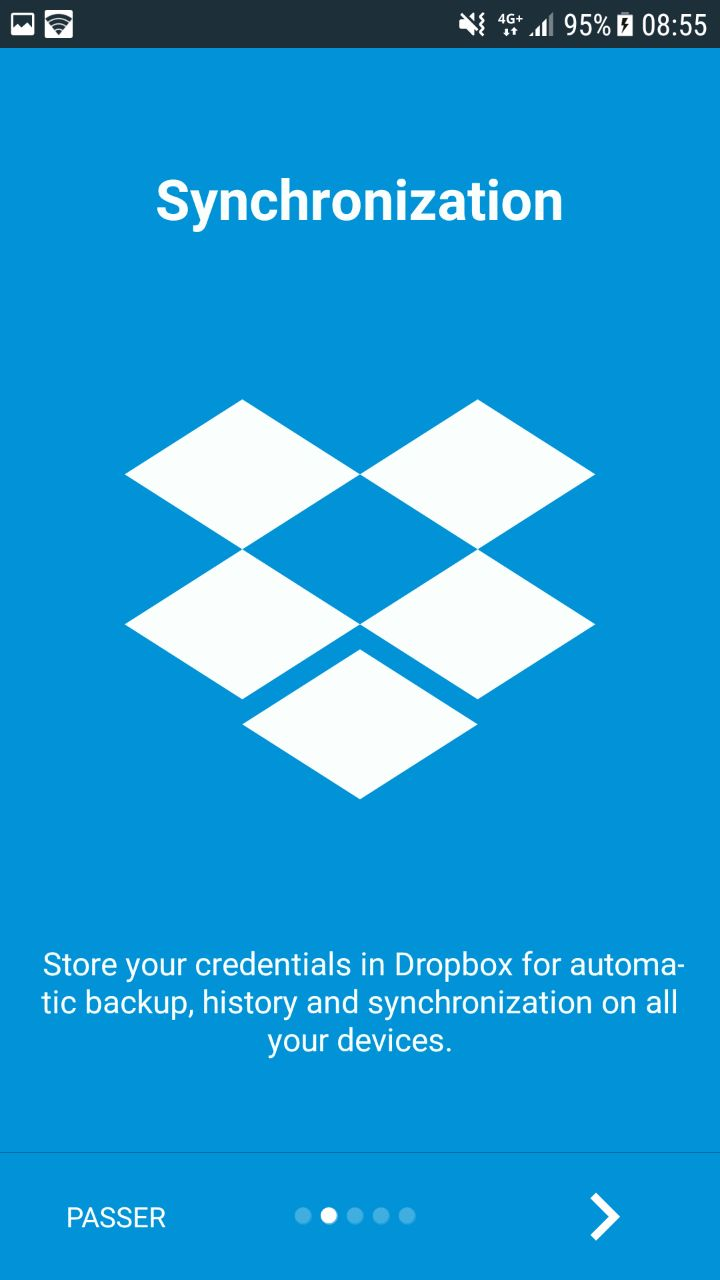
\includegraphics[width=.2\textwidth]{intro-2.jpg}
% 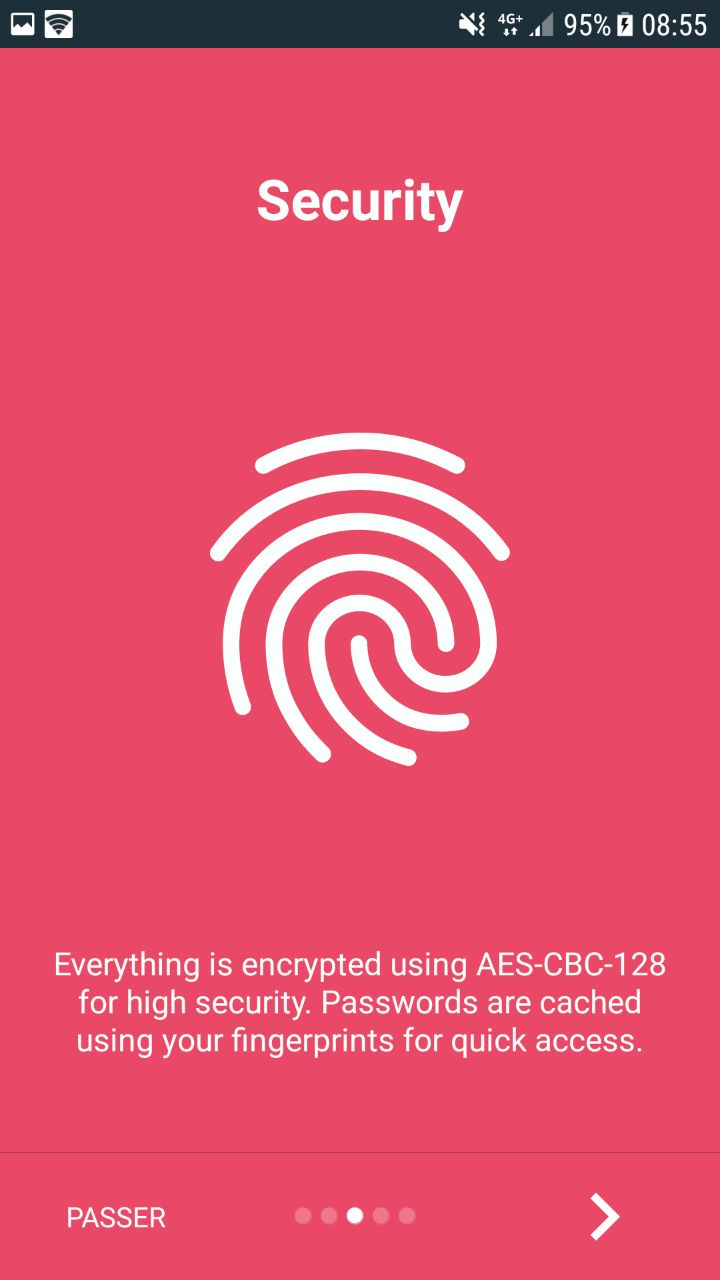
\includegraphics[width=.2\textwidth]{intro-3.jpg}
% 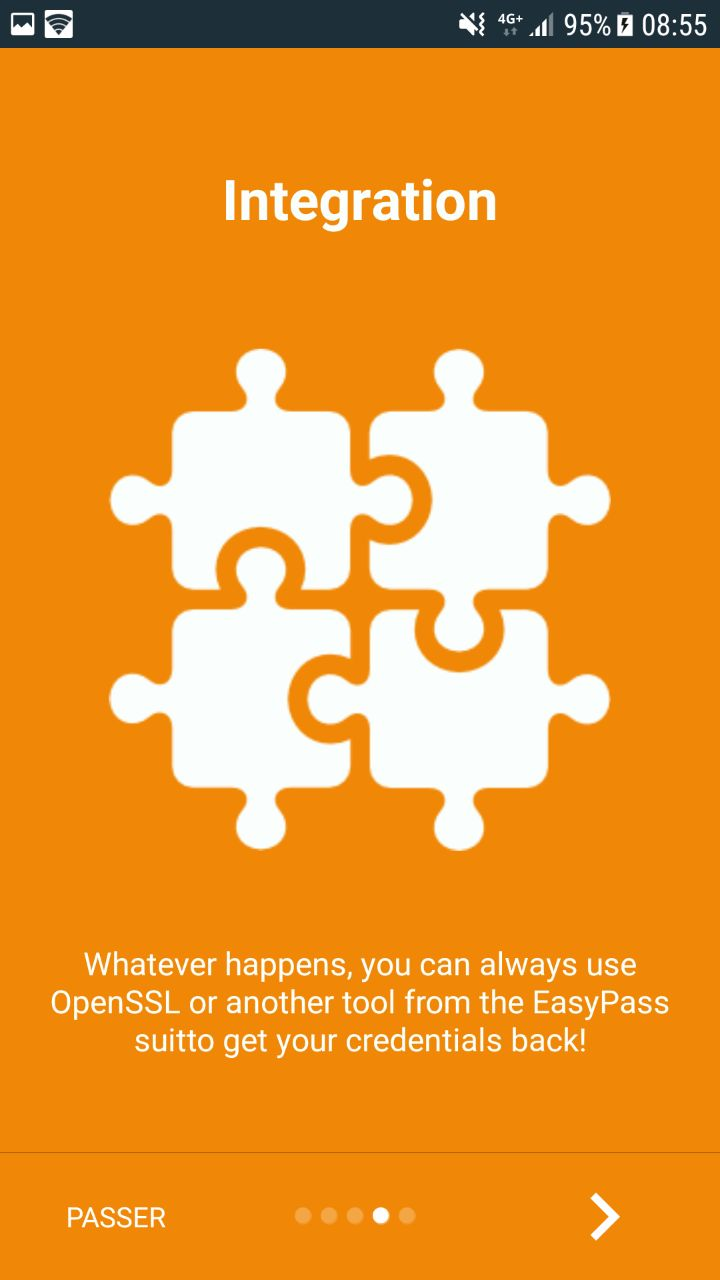
\includegraphics[width=.2\textwidth]{intro-4.jpg}
% 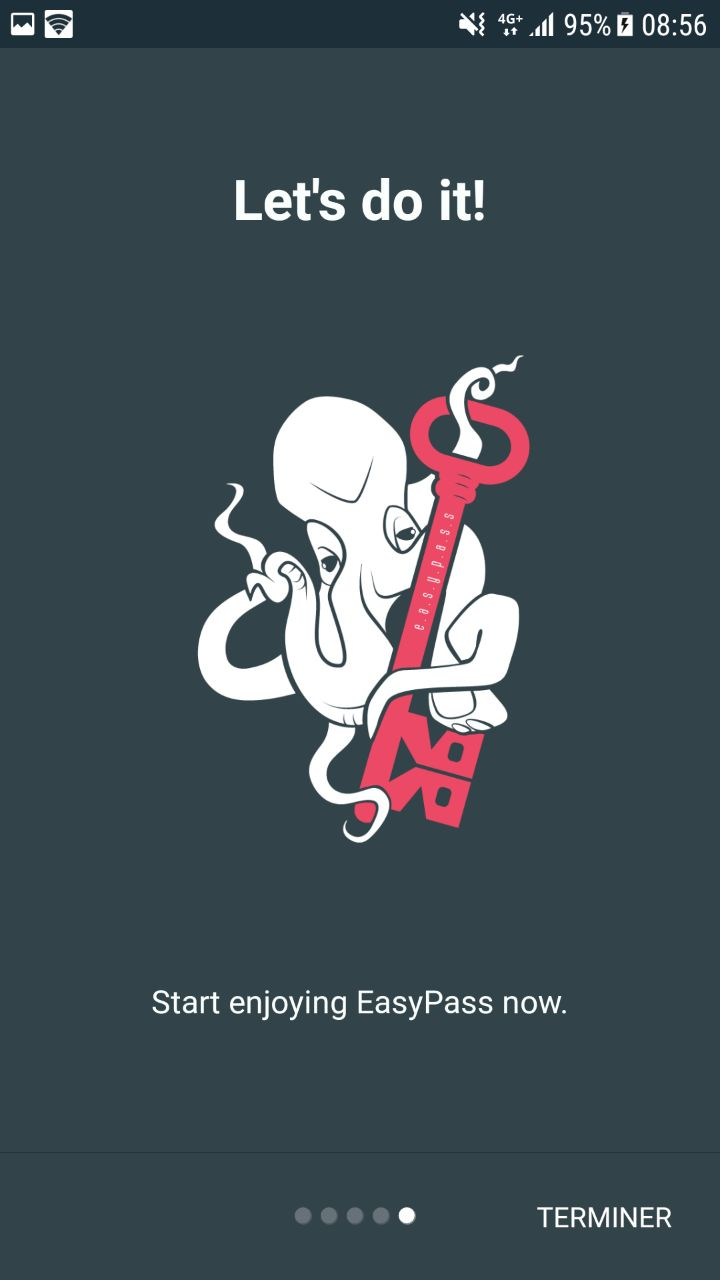
\includegraphics[width=.2\textwidth]{intro-5.jpg}



\section{Vocabulaire}

Dans ce document, nous utiliserons les termes suivants:

\begin{description}
    \item[compte/account] un ensemble d'information concernant un mot de passe: nom, email, pseudo, notes, date de création, date de modification;
    \item[session] un fichier contenant un ensemble de comptes, sécurisé par un mot de passe unique;
    \item[master password] un mot de passe permettant de décrypter une session.
\end{description}


% Fonctionnalités de base:

% \begin{itemize}
%     \item liste des comptes (une seule session);
%     \item opérations CRUD sur un compte;
%     \item synchronisation de la session au format json sur Dropbox;
%     \item cryptage AES CBC de la session avec mot de passe;
%     \item décryptage de la session via \emph{fingerprint} ou \emph{pattern};
%     \item raccourcis pour copier rapidement une information de compte (mot de passe, email, pseudo);
%     \item fonctionnalité de recherche via mot-clés; 
% \end{itemize}

% Fonctionnalités optionnelles (\emph{nice to have}):

% \begin{itemize}
%     \item (implémenté) sécursation de l'application: pas de capture d'écran ni de preview dans les \emph{recents};
%     \item (implémenté) générateur de mot de passe;
%     \item historique des mots de passe pour un compte;
%     \item gestion des duplicats; 
%     \item feedbacks visuels concernant la sécurité des mots de passe: \emph{weak, OK, strong};
%     \item support d'autres plateformes que Dropbox (Google Drive, etc.);
%     \item portage sur IOS;
% \end{itemize}
